\input{header.tex}
% this file declares acronyms. There are two classes: abbrev for abbreviations and nomencl for nomenclature

\acsetup{
  first-style=short
}

% class `abbrev': abbreviations:
\DeclareAcronym{CE}{
  short = CE ,
  long  = contractile element ,
  class = abbrev
}
\DeclareAcronym{SEE}{
  short = SEE ,
  long  = serial elastic element ,
  class = abbrev
}
\DeclareAcronym{PEE}{
  short = PEE ,
  long  = parallel elastic element ,
  class = abbrev
}
\DeclareAcronym{SDE}{
  short = SDE ,
  long  = serial damping element ,
  class = abbrev
}
\DeclareAcronym{MTU}{
  short = MTU ,
  long  = muscle tendon unit ,
  class = abbrev
}

% class `nomencl': nomenclature
\DeclareAcronym{angelsperarea}{
  short = \ensuremath{a} ,
  long  = The number of angels per unit area ,
  sort  = a ,
  class = nomencl
}
\DeclareAcronym{numofangels}{
  short = \ensuremath{N} ,
  long  = The number of angels per needle point ,
  sort  = N ,
  class = nomencl
}
\DeclareAcronym{areaofneedle}{
  short = \ensuremath{A} ,
  long  = The area of the needle point ,
  sort  = A ,
  class = nomencl
}

% usage: \ac{ny}, \ac{la} and \ac{un} are abbreviations 
%        whereas \ac{angelsperarea}, \ac{numofangels} and \ac{areaofneedle} are part of the nomenclature


\graphicspath{
{images/summer_school_study/png/}
{images/summer_school_study/}
{images/summer_school_study/plots/}
{images/summer_school_study/2018/}
{images/fiber_creation/}
{images/motor_unit_assignment/}
}

\begin{document}

\newcommand{\opendihu}{OpenDiHu}.
\newcommand{\Opendihu}{OpenDiHu}.
 
%\setcounter{tocdepth}{2}
\tableofcontents
%\newpage


%\part{Introduction}
%  \chapter{Motivation}
%  - great picture, digital human vision, connection to soft tissue robotics\\
%  - EMG, parameter estimation, see motivation of IRTG paper\\
%  - MU estimation\\
%  
%  \chapter{State of the art and aims}
%  \chapter{Own contributions}
%  - own contributions
%  \chapter{Overview}
%  - structure of following sections
\part{Digital human}

%\input{02_comparative_study}

% \chapter{Formulation of electrophysiology and muscle contraction}
%    - electrophysiology introduction
%    \section{State of the art}
%    - Hodgkin-Huxley, shorten, advanced models, how it gets solved
%    \section{discretization}
%    - discretization of electrophysiology, operator splitting
%    \section{Standard for formulation of models}
%    - cellml introduction
%    \section{Bidomain}
%    - EMG
%    \section{Multidomain}
%    - multidomain formulation
%    \section{Formulation of solid mechanics}
%    - basics solid mechanics framework, material modeling, 
%    
%    \section{Simulation workflow}
%    - simulation workflow of skeletal muscle
%  
% \chapter{Numerics}
%   \section{Fundamentals of the discretization}
%    \section{Finite element method}
%    - basics FEM formulation of Laplace operator and diffusion equation, boundary conditions
%    \section{Incompressible nonlinear solid mechanics}
%    - incompressibility, penalty formulation vs. mixed formulation\\
%    - governing nonlinear eq.\\
%    - jacobian
%   \section{Numerical schemes}
%    \section{time stepping schemes}
%    \section{linear system solvers}
%    \section{newton algorithm}
%  % 
% \chapter{Simulation software}
%    \section{State of the art}
%    - review on bioengineering simulation frameworks 
%    
%    \section{OpenCMISS}
%  - OpenCMISS introduction, iron zinc cmgui, unstructured\\
%  
%  - Strang splitting, solvers 1D\\
%  - improved interpolation\\
%  - parallelization, issue with 1D \\
%  - 3D parallelization strategies\\
%  - design flaws, memory\\
%    % untergliedern, z.B. schnittstellen parall etc.
%    \section{The simulation framework \emph{opendihu}}
%    - modularity of opendihu, concepts (python c++ build system)
%    \section{Overview of discretization features}
%    - feature overview, implemented equations, ansatz functions, meshes
%    \section{Input and output}
%    - file i/o parallel, i: only local data important for high parallelism, o: paraview
%    \section{In-situ visualization}
%    - in-situ
%    \section{Details on the implementation}
%    \section{Representation of structured meshes}
%    \section{Parallel data handling}
%    - data structures, petsc variables, partitioning, ghost communication
%    \section{Implementation of boundary conditions}
%    - Neumann, Dirichlet boundary conditions
%    \section{Implementation of material formulation and automatic derivation of derivatives}
%    - implementation of solid mechanics with analytic differentiation
%    
%    \section{efficient and configurable data transfer}
%    - data layout details, efficient transfer of variables between solvers
%    \section{Mapping between meshes}
%    - parallel mapping between meshes, invertability of index space represesantion
%    \section{An efficient solver to the Monodomain equation}    
%    - cellml code generator and its optimizations - openmp, simd, vc
%    \section{Details on the partitioning}
%    - fibers emg structure and partitioning
%    \section{Parallelization of the multidomain system}
%    - multidomain parallelization, reordering of matrix
%    \section{load balancing}
%    - load balancing on fiber level
% \chapter{External coupling}
%    - introduction to external coupling, precice
%    \section{coupling with FEBio}
%    \section{coupling with AceFEM}
%  

\chapter{Muscle Fibers and Motor Units}
\section{Introduction}
requirements
We identify two different sets of requirements 
two different approaches
1. given set of fibers in a 2D grid, assign to Mus
2. select fibers from this grid for MUs
\section{Related Works}

\section{Method 1: Assignment of a Given Set of Fibers to Motor Units}
\subsection{Stochastic Formulation and Algorithm}\label{sec:stochastic_formulation_and_algorithm}

At first, for each fiber ${(i,j)}$ in a two-dimensional grid the probabilities $p(i,j,k_\text{MU})$ to be part of a specific MU $k_\text{MU}$ are computed. Then, in a sampling step, the actual assignments of MUs to the fibers is performed.

The following conditions are enforced on the probabilities. (i) The probabilities have to be valid, i.e., positive and for all MUs at any fiber they sum up to 1. (ii) The sizes of the motor units have to following an exponential progression $q$, with  MU 1 containing the least and MU $n_\text{MU}$ having the most fibers. (iii) For any given MU the spatial arrangement of its fibers in the cross-sectional plane is described by a radial kernel function $\hat{p}$. The fiber density of the MU increases when moving closer to a given center point.

Condition (iii) approximates the fact that the fibers of a MU are located in proximity, forming the MU territory.

The exponential progression of condition (ii) is defined to follow the following function:
%
\begin{align}\label{eq:mus_q}
  q(k_\text{MU}) = b^{k_\text{MU}} / \s{\ell=1}{n_\text{MU}} b^\ell.
\end{align}
%
% f(x) = 1/(1+a*x^2),  ∫f(x)dx = arctan(sqrt(x)*x)/sqrt(a) + c
% stddev = sqrt(variance) = sqrt(∫{-∞,+∞} (f(x)-0)^2 dx) = sqrt(pi/(2*sqrt(a)))
% => a = pi^2 / (4*\sigma^4)
%
% 
The basis $b$ should be set to a value greater than one, e.g., $b=\num{1.2}$.

For condition (iii), center positions $\bfx_{k_\text{MU}}, k_\text{MU}=1, \dots, n_\text{MU}$ of the MU territories are defined. 
For this purpose, the muscular cross-section is approximated by a regular grid of $n \times n$ fibers. The center positions are quasirandomly selected inside the inner 80\% of this quadratic domain. The outer border with width of 10\% is not considered because the points should not be at the border of any MU territory but rather at their center.

The used quasirandom sequence is the following Weyl low-discrepancy sequence \cite{Weyl1916}:
\begin{align*}
  &x_0 = (n+1)/2, \quad &&y_0 = (n+1)/2,\\[4mm]
  &x_{i} = x_0+(i\cdot \alpha_1) \mod \num{1.0},
  &&y_{i} = y_0+(i\cdot \alpha_2) \mod \num{1.0},\\[4mm]
  &\alpha_1 = \num{0.5545497}, \quad &&\alpha_2 = \num{0.308517}.
\end{align*}
It is known that the sequences $x_i$ and $y_i$ are equidistributed in $[0,1)$ for any irrational $\alpha_1$ and $\alpha_2$ \cite{Weyl1916}. The chosen values lead to a sequence of 2D points $(x,y)\in $$[0,1)^2$ with low discrepancy and a good coverage of the domain for any number $n^2$ of fibers. Accordingly, the MU territory center points are defined as $\bfx_{k_\text{MU}} = (x_{k_\text{MU}}, y_{k_\text{MU}})^\top$.

The radial kernel function $\hat{p}$ for a given MU $k_\text{MU}$ is defined as follows.
\begin{align}\label{eq:phat_kernel}
  \hat{p}(i,j,k_\text{MU}) = \dfrac{1}{1 + a\,\vert\bfx_{k_\text{MU}} - \bfx_{i,j}\vert^2}, \quad \text{with }a = \dfrac{\pi^2}{4\sigma^4}.
\end{align}
The coordinates $i$ and $j$ specify the grid point $\bfx_{i,j} = (i,j)^\top$ of the fiber. The factor $a$ is computed from the given standard deviation $\sigma$ of the spatial distribution of the MU territory around the center point. A lower value of $\sigma$ leads to smaller and \say{sharper} MU territories, for higher values of $\sigma$ the MU territories mix with each other.
This form of kernel function was chosen because it can be computed efficiently unlike, e.g., a Gaussian kernel function.

If the kernel function in \cref{eq:phat_kernel} is used to describe the probability of fiber $(i,j)$ to be in MU $k_\text{MU}$, the conditions (ii) and (i) will not be fulfilled. Instead, a derived term $p(i,j,k_\text{MU})$ is used that satisfies the requirements.
For condition (ii), additional scalar factors $\lambda_k, k=1\dots n_\text{MU}$ are introduced for the MUs that yield the required exponential distribution.
For condition (i), the term is normalized by the respective division. The resulting formulation is given as follows,
\begin{align}\label{eq:mu_p}
  p(i,j,k_\text{MU};\{\lambda_k\}_{1\dots n_\text{MU}}) = \dfrac{\hat{p}(i,j,k_\text{MU}) \cdot \lambda_{k_\text{MU}}}{\s{\ell_\text{MU}=1}{n_\text{MU}} \hat{p}(i,j,\ell_\text{MU}) \cdot \lambda_{\ell_\text{MU}}}.
\end{align}
Here, the factors $\{\lambda_k\}_{1\dots n_\text{MU}})$ are to be determined. Setting $\lambda_{k_\text{MU}} = q(k_\text{MU})$ would not yield the required exponential distribution of probabilities, because the MU center points $\bfx_{k_\text{MU}}$ have varying distances between each other and therefore the accumulated propabilities of the total set of fibers to be part of a particular MU $k_\text{MU}$ are different for each MU, even before scaling with the factors $\{\lambda_k\}$.
Therefore, the value of the factors has to be determined by solving an optimization problem.

The objective function to be minimized is given by%
\begin{align}\label{eq:mus_objective}
  F(\{\lambda_k\}_{1\dots n_\text{MU}}) = \s{k_\text{MU}=1}{n_\text{MU}} \left(q(k_\text{MU}) - \s{i=1}{n}\s{j=1}{n}p(i,j,k_\text{MU};\{\lambda_k\}_{1\dots n_\text{MU}}) / n^2\right)^2.
\end{align}
It sums up the quadratic error for every MU between the desired propability $q(k_\text{MU})$ per fiber and the achieved probability per fiber under the current value of the scaling factors $\lambda_k$. The achieved probability is computed by a double sum over all fibers $(i,j)$ and the formulated probability function $p$ divided by $n^2$ to get the value per fiber.
After solving the optimization problem and plugging the factors $\{\lambda_k\}$ into \cref{eq:mu_p} we get every probability for a fiber to be in a MU by \cref{eq:mu_p}.

Drawing samples $Y$ with the given probabilities in order to assign actual MU numbers to every fiber is done using inverse transform sampling. The inverse cumulative distribution function (CDF) $F_q^{-1}(k_\text{MU})$ is applied onto a random value $X$ drawn from a continuous uniform distribution $\mathcal{U}$:
\begin{align*}
  Y = F_q^{-1}(X)\quad \text{with }X\sim \mathcal{U}\big(0,F_q(n_\text{MU})\big), \quad F_q(k_\text{MU}) = \s{\ell_\text{MU}=1}{k_\text{MU}} p(i,j,\ell_\text{MU}).
\end{align*}
Computing the inverse of the CDF is computationally cheap as the probabilities are discrete and, thus, a loop over the values of the CDF suffices.

To reduce outliers during the sampling where some MUs get zero, exceptionally little or exceptionally many fibers assigned, the sampling procedure is performed five times.
A histogram with bins for the MUs is computed and provides the number of fibers per MUs. For all MUs $k$ that have zero fibers assigned, the one fiber where the probability for the respective MU $k$ is highest is determined. This is usually the fiber closest to the center point $\bfx_k$ of the MU $k$. The MU assignment of this fiber is changed to $k$, such that the MU $k$ is no longer empty but has one fiber.

In every of the five iterations, the squared error between the sampled MU sizes and the predicted sizes given as $q(k_\text{MU})\cdot n^2$ is computed and the best result is used for the final MU assignments.

\subsection{Algorithm to Solve the Optimization Problem}
The problem to be solved can be stated as %
\begin{align*}
  \text{``Find}\quad \{\lambda_k\}_{1\dots n_\text{MU}} \text{ with } \lambda_k > 0 \quad \text{ s.t. } \quad F(\{\lambda_k\}_{1\dots n_\text{MU}}) \quad \text{ is minimal'',}
\end{align*}
with the objective function $F$ given in \cref{eq:mus_objective}. The solution is obtained by a Quasi-Newton method, more specifically the limited-memory version of the \emph{Broyden–}~\emph{Fletcher–}~\emph{Goldfarb–}~\emph{Shanno} algorithm with box constraints by the authors of \cite{byrd1995limited}. The Fortran implementation is made accessible in Python by the \emph{SciPy Optimize} package.

With increasing number $n^2$ of fibers and increasing number $n_\text{MU}$ of MUs the evaluation duration for the objective function and the number of optimization parameters increases. For numbers about $n^2 > 1000$ and $n_\text{MU} > 25$ the solution times become unfeasible.

As a remedy we develop an algorithm to split the large optimization problem into multiple smaller ones which reduces the total runtime. 
The set of factors $\{\lambda_k\}_{1\dots n_\text{MU}}$ is partitioned into chunks, i.e., subsets of given size $n_\text{per\_chunk}$ leading to a total of $n_\text{chunks} = \lceil n_\text{MU} / n_\text{per\_chunk} \rceil$ chunks.
(Remainder chunks at the end may have one set element less.)
The factors for chunk no. $c$ are selected in a strided manner, as $\{\lambda_k\}$ with indices ${k=c, c+n_\text{chunks}, c+2\,n_\text{chunks}, \dots}$.

A number of subsequent optimization problems is solved where the optimization parameters are each time given by individual chunks.
Initially, all scalar factors $\lambda_k$ are set to one. After each solved optimization problem, the $\lambda_k$ values are updated with the found minimizer.
In this loop over all chunks, the number $n_\text{factors\_up\_to\_chunk}$ of already solved scalar factors up to the current iteration starts with zero and increases by $n_\text{per\_chunk}$ after each iteration, finally arriving at $n_\text{MU}$ after the last iteration.

These smaller optimization problems have a similar formulation as the overall problem, given by \cref{eq:mus_q,eq:mu_p,eq:mus_objective}. The number $n_\text{MU}$ of motor units in \cref{eq:mu_p,eq:mus_objective} is replaced by the number $n_\text{factors\_up\_to\_chunk}+n_\text{per\_chunk}$ of factors that will be solved after the current iteration. The argument of the objective in \cref{eq:mus_objective} contains only the $n_\text{per\_chunk}$ factors of the current chunk, which will be determined in the current iteration. The $n_\text{factors\_up\_to\_chunk}$ factors in the definition that are not given by the argument of the objective are set to the solutions obtained in previous iterations.

The indexing of the MU center positions $\bfx_{k_\text{MU}}$ is adjusted such that only the MUs up to and including the current chunk are considered. The indexing in the exponential progression formulated by \cref{eq:mus_q}, however, stays the same, here the argument $k_\text{MU}$ of the function $q$ refers to the initial MU number.

In summary, the considered setting contains an increasing number of MUs with every iteration. The number of optimization parameters and, thus, new MUs is kept constant while the number of summands in the objective function increases. In consequence, the evaluation of the objective function gets more expensive with increasing iteration number while the size of the optimization problem stays constant.

\section{Method 2: Selection of Fibers and Assignment to Motor Units}

The second method proceeds similar to the first method in that at first the probability for a specific MU is defined for any fiber $(i,j)$ in the $n \times n$ grid. Then the actual MU assignments are sampled from the probability distributions. The difference to the first method is that any fiber is also allowed to not be assigned to any MU. This makes the definition of the probabilities easier and no optimization is required.

The three conditions defined in \cref{sec:stochastic_formulation_and_algorithm} are also imposed for the second method. The definition of the MU center positions $\bfx_{k_{MU}}$ follows the same low-discrepancy series. Also, the radial kernel function \cref{eq:phat_kernel} can be reused to describe the spatial distribution of probability for a given MU. Instead of \cref{eq:mu_p}, the probability is formulated directly as the product of the kernel function $\hat{p}$ and the exponential progression $q$:
\begin{align*}
  \tilde{p}(i,j,k_\text{MU}) = \hat{p}(i,j,k_\text{MU}) \cdot q(k_\text{MU}).
\end{align*}
%
To ensure that the function is within the bounds of a probability, $p \leq 1$, the result is divided by the maximum occuring value,%
\begin{align*}
  p(i,j,k_\text{MU}) = \dfrac{\tilde{p}(i,j,k_\text{MU})}{\max\limits_{\substack{\bar{i},\bar{j} = 1,\dots,n\\\bar{k}_\text{MU}=1,\dots,n_\text{MU}}} \tilde{p}(\bar{i},\bar{j},\bar{k}_\text{MU})}.
\end{align*}
%

In the sampling step, for every fiber $(i,j)$ the probabilities $p(i,j,k_\text{MU}), k_\text{MU}=1,\dots,n_\text{MU}$ for the MUs and the remaining probability $\bar{p} = 1-\sum_{k_\text{MU}} p(i,j,k_\text{MU})$ is computed. The 

\section{Results and Discussion}


\begin{figure}%
  \centering%
  \includegraphics[width=0.8\textwidth]{images/motor_unit_assignment/MU_fibre_distribution_13x13_10_fiber_distribution.pdf}%
  \caption{a.}%
  \label{fig:MU_fibre_distribution_13x13_10_fiber_distribution}%
\end{figure}

\begin{figure}%
  \centering%
  \begin{subfigure}[t]{0.48\textwidth}%
    \centering%
    \includegraphics[width=\textwidth]{images/motor_unit_assignment/MU_fibre_distribution_13x13_10_2d_fiber_distribution.pdf}%
    \caption{$\sigma = n/10 = 1.3$}%
    \label{fig:MU_fibre_distribution_13x13_10_2d_fiber_distribution}%
  \end{subfigure}
  \begin{subfigure}[t]{0.48\textwidth}%
    \centering%
    \includegraphics[width=\textwidth]{images/motor_unit_assignment/MU_fibre_distribution_13x13_10_2d_fiber_distribution_sigma.pdf}%
    \caption{$\sigma = n/100 = 0.13$}%
    \label{fig:MU_fibre_distribution_13x13_10_2d_fiber_distribution_sigma}%
  \end{subfigure}
  \begin{subfigure}[t]{0.48\textwidth}%
    \centering%
    \includegraphics[width=\textwidth]{images/motor_unit_assignment/MU_fibre_distribution_sparse_13x13_10_2d_fiber_distribution.pdf}%
    \caption{$\sigma = n/10 = 1.3$, 115 of 169 fibers, i.e. 68\% have no motor unit.}%
    \label{fig:MU_fibre_distribution_sparse_13x13_10_2d_fiber_distribution}%
  \end{subfigure}
  \begin{subfigure}[t]{0.48\textwidth}%
    \centering%
    \includegraphics[width=\textwidth]{images/motor_unit_assignment/MU_fibre_distribution_sparse_13x13_10_sigma_2d_fiber_distribution.pdf}%
    \caption{$\sigma = n/100 = 0.13$, 106 of 169 fibers, i.e. 63\% have no motor unit}%
    \label{fig:MU_fibre_distribution_sparse_13x13_10_sigma_2d_fiber_distribution}%
  \end{subfigure}
  \caption{a.}%
  \label{fig:extraction_result}%
\end{figure}%

\begin{figure}%
  \centering%
  \includegraphics[width=0.8\textwidth]{images/motor_unit_assignment/MU_fibre_distribution_13x13_10_pdf.pdf}%
  \caption{a.}%
  \label{fig:MU_fibre_distribution_13x13_10_pdf}%
\end{figure}

\begin{figure}%
  \centering%
  \begin{subfigure}[t]{0.31\textwidth}%
    \centering%
    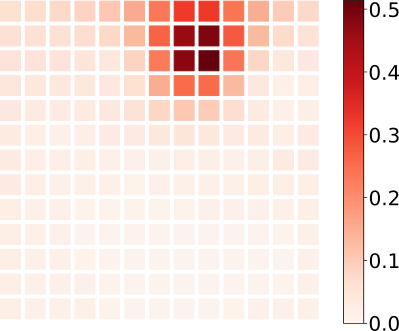
\includegraphics[width=\textwidth]{images/motor_unit_assignment/MU_fibre_distribution_13x13_10_fibers_mu3.pdf}%
    \caption{.}%
    \label{fig:MU_fibre_distribution_13x13_10_fibers_mu3}%
  \end{subfigure}
  \quad
  \begin{subfigure}[t]{0.31\textwidth}%
    \centering%
    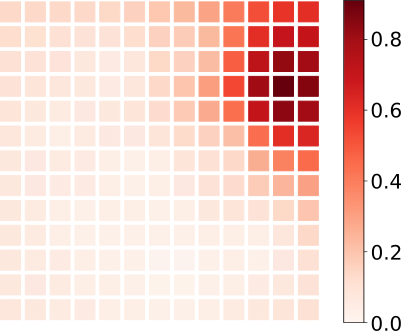
\includegraphics[width=\textwidth]{images/motor_unit_assignment/MU_fibre_distribution_13x13_10_fibers_mu9.pdf}%
    \caption{.}%
    \label{fig:MU_fibre_distribution_13x13_10_fibers_mu9}%
  \end{subfigure}
  \quad
  \begin{subfigure}[t]{0.31\textwidth}%
    \centering%
    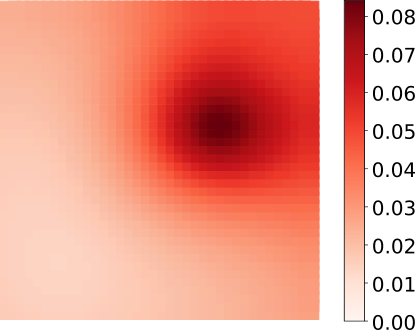
\includegraphics[width=\textwidth]{images/motor_unit_assignment/MU_fibre_distribution_37x37_50_fibers_mu41.pdf}%
    \caption{$\sigma = n/100 = 0.13$}%
    \label{fig:MU_fibre_distribution_37x37_50_fibers_mu41}%
  \end{subfigure}
  \caption{a.}%
  \label{fig:extraction_result}%
\end{figure}%

\begin{figure}%
  \centering%
  \begin{subfigure}[t]{0.48\textwidth}%
    \centering%
    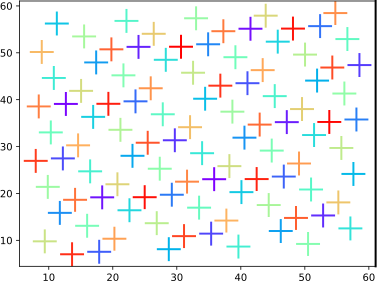
\includegraphics[width=\textwidth]{images/motor_unit_assignment/MU_fibre_distribution_67x67_100_mu_positions.pdf}%
    \caption{.}%
    \label{fig:MU_fibre_distribution_67x67_100_mu_positions}%
  \end{subfigure}
  \quad
  \begin{subfigure}[t]{0.48\textwidth}%
    \centering%
    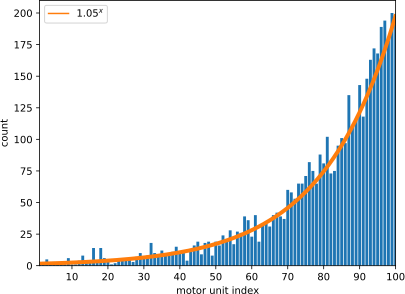
\includegraphics[width=\textwidth]{images/motor_unit_assignment/MU_fibre_distribution_67x67_100_fiber_distribution.pdf}%
    \caption{.}%
    \label{fig:MU_fibre_distribution_67x67_100_fiber_distribution}%
  \end{subfigure}
  \begin{subfigure}[t]{0.48\textwidth}%
    \centering%
    \includegraphics[width=\textwidth]{images/motor_unit_assignment/MU_fibre_distribution_67x67_100_2d_fiber_distribution.pdf}%
    \caption{.}%
    \label{fig:MU_fibre_distribution_67x67_100_2d_fiber_distribution}%
  \end{subfigure}
  \quad
  \begin{subfigure}[t]{0.48\textwidth}%
    \centering%
    \includegraphics[width=\textwidth]{images/motor_unit_assignment/MU_fibre_distribution_sparse_67x67_100_2d_fiber_distribution.pdf}%
    \caption{.}%
    \label{fig:MU_fibre_distribution_sparse_67x67_100_2d_fiber_distribution}%
  \end{subfigure}
  \caption{a.}%
  \label{fig:extraction_result}%
\end{figure}%

%  \chapter{An algorithm for mesh generation}
%    - introduction, need for fiber and 3d mesh
%    \section{State of the art}
%    - literature, laplace potential flow idea
%    \section{Data preprocessing}
%    - visual human dataset, methods to extract surface, approximation by spline surfaces
%    \section{Outline of the algorithm}
%    - pseudo code
%    \section{Plane mesh smoothing}
%    \section{Parallelization}
%    \section{Generation of fiber meshes}
%    - generation of muscle mesh, 3D and fibers, also in parallel
%  
% \chapter{Simulation scenarios}
%    \section{Simulation of electromyography with fiber-based formulation}
%      - scenario static-biceps-emg, composite meshes
%    \section{Simulation of electromyography with multidomain formulation}
%    \section{Muscle contraction with fiber-based formulation}
%      - fibers with contraction
%    \section{Muscle contraction with multidomain formulation}
% \chapter{Technical simulation results}
%    \section{Runtime evaluation}
%    - results and experiments, runtime, peak performance\\
%    - monodomain runtime comparison OpenCMISS opendihu
%    \section{parallel partitioning}
%    - parallel partitioning and weak scaling, opencmiss and opendihu 
%    \section{memory consumption}
%    - memory scaling OpenCMISS
% \chapter{biomechanical simulation results}
%    \section{Simulation of fatigue}
%    - monodomain, hh  shorten, fatigue effects
%    \section{Simulation of EMG}
%    - static biceps emg\\
%    - fibers with contraction\\
%    - multidomain with fat layer\\
%    - multidomain with contraction\\
%
%\part{Soft tissue robotics}
%\chapter{...}
%  - introduction, handling flexible objects, overview of different object types\\
%  - basics Lagrange formulation of cable\\
%  - cable with friction on surface\\
%  - placing cable\\
%  - peg-in-hole, with sparse grids\\
%  - simulation of 2d tissue\\
%  - gripping point estimation\\
%  
%  \cite{Maier2021}
%  
%\part{Conclusion}

% -------------- Literaturseite --------------------
\newpage

%\acsetup{pages/display=first,pages/name=true}

% Abbreviations
\printacronyms[include-classes=abbrev,name=Abbreviations]

% Nomenclature
\printacronyms[include-classes=nomencl,name=Nomenclature]


%\bibliography{references}{}
%\bibliographystyle{abbrv}
\printbibliography[%
  % change title
  title=Bibliography
]


% -------------- Anhang ------------
%\appendix
%\input{8_anhang.tex}

\end{document}

%\input{preambule/footer}
